\section{Sprint 1: Generación de perfil de datos personales}

\subsection{Planificación}
\begin{itemize}
    \item \textbf{Inicio}: 28 de abril del 2015.
    \item \textbf{Fin}: 19 de mayo del 2015.
\end{itemize}

\subsection{Descripción}
En este sprint se realizará la sección del perfil del usuario, para lo cual se deberá definir en el backend, las clases Profile y Gender, así como los recursos para acceder a ellas a través de la API. Además se realizara la documentación correspondiente para su consumo.
Por parte del frontend se debe desarrollar los recursos de acceso a la API, las vista HTML y cada uno de sus controladores: Una para mostrar el perfil y otra de edición del mismo.

Para lograr brindarle esta funcionalidad se desarrollarán los formularios de carga y edición para permitirle gestionar su información en el momento que lo desee.

\subsection{User Stories relacionados}
{\scriptsize
\begin{table}[h]
	\begin{tabular}{|l|p{10cm}|c|}
	\hline
        \multicolumn{1}{|c|}{\textbf{ID}} &
        \multicolumn{1}{|c|}{\textbf{Enunciado de la historia}} &
        \textbf{Prioridad} \\     
    \hline
        US-\ref{infoPerfil} &
        Como paciente quiero cargar mi información personal nombre, apellido, fecha de nacimiento y más para armar mi perfil e identificarme así en el sistema.& Alta
        \\
    \hline 
	 \end{tabular}
\end{table}
}




\subsection{Modelo de datos}

El Diagrama que propio de este sprint se puede ver en la \textbf{Figura \ref{modeloEspecifico}}, allí se indican exactamente las clases que se usarán en este sprint y que serán detalladas con detenimiento en el presente documento. Se recuerda que se ha realizado un Diagrama de clases tentativo que se puede ver en la \textbf{Figura \ref{2-modelo_datos_general}}, dicho diagrama  será utilizado como base para este sprint y posee un alcance limitado el cual se irá modificando a medida que se profundice en los temas.



\begin{figure}[h]
  \centering
  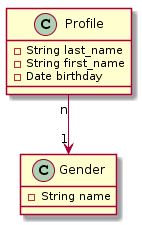
\includegraphics[width=.2\textwidth]{img/tp1_parte2/1-modelo_dato_especifico}
  \caption{Modelo de datos Específico}
  \label{modeloEspecifico}
\end{figure}
\clearpage

\subsection{Descripción de las Clases}

    \subsubsection{Clase Profile}
    Dicha clase hace referencia a los datos que caracterizan al perfil del usuario.

    \textbf{Descripción de los atributos}
    \begin{itemize}
            \item \textbf{id:}Identificador único del perfil(tipo int)
			\item\textbf{ last\_name 	:}	Apellido de la persona(tipo string).
			\item \textbf{ first\_name: } 	Nombre de la persona (tipo string).
			\item \textbf{birthday 	:}	Fecha de nacimiento de la persona, en formato ISO 8601 (tipo datetime).
			\item \textbf{gender\_id:} 	Identificador único del género asociado 	(tipo int).
    \end{itemize} 
	\textbf{Dirección del recurso:}
    \begin{lstlisting}[language=json,firstnumber=1]
    <BASE URL>/profiles/{:id}
    \end{lstlisting}

    \textbf{Json generado por la API}    
    \begin{lstlisting}[language=json,firstnumber=1]
    {
    "resource": 
    {
    "id": 1,
    "gender": 
    {
    "id": 1,
    "name": "Masculino",
    "description": null
    },
    "birthday": "1990-10-26",
    "last_name": "Terreno",
    "first_name": "Milton"
    }
    }
    \end{lstlisting}

\subsubsection{Clase Gender} 
    \textbf{Descripción de los atributos}
	\begin{itemize}
            \item \textbf{name :}	Nombre del género (tipo string).
            \item \textbf{description 	:}	Descripción del género (tipo string).
    \end{itemize} 
    
    \textbf{Dirección del recurso:}
    \begin{lstlisting}[language=json,firstnumber=1]
    <BASE URL>/genders
    \end{lstlisting}

    \textbf{Json generado por la API}    
        \begin{lstlisting}[language=json,firstnumber=1]
{
    "resource": 
[
{
    "id": 1,
    "name": "Masculino",
    "description": null
},
        {
            "id": 2,
            "name": "Femenino",
            "description": null
        }
    ]
}
        \end{lstlisting}

\subsection{Modelo Funcional}
Se describirán las funciones usando como marco de apoyo el sprint Backlog, además se armará el diagrama de casos de uso del presente Sprint \textbf{[Figura \ref{1-caso_de_uso}]} que irá creciendo  medida se vaya avanzando en el proyecto.
    \begin{figure}[h]
        \centering
        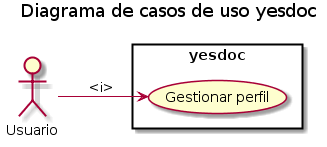
\includegraphics[width=0.5\textwidth]{img/tp1_parte2/1-caso_de_uso}
        \caption{formulario de edición de perfil}
		\label{1-caso_de_uso}
    \end{figure}
	{\scriptsize
	\begin{center} %sidewaystable
	\centering
	%\begin{adjustbox}{max width=\textheight}
    \resizebox{\textwidth}{!}{
	\begin{tabular}{|l|l|l|l|}
	    \hline
	        \textbf{Area a cargo} &
	        \textbf{Responsable} &        
	        \textbf{Tarea} &
	        \textbf{US} \\
	    \hline
	    Front-end & Yanina Morales&  Generación de plantilla principal, con logo, botonera y colores  & US-\ref{resumenInfo} \\ \hline
	    Front-end& Iván Terreno & Generación de controladores para consumir Json de la Api  & US-\ref{resumenInfo} \& US-\ref{infoSalud} \\ \hline
        Front-end& Iván Terreno & Capacitación sobre las ventajas de usar resource frente a http & US-\ref{resumenInfo} \& US-\ref{infoSalud}\\ \hline
        Front-end&Iván Terreno  & Creación de página de perfil&  US-\ref{resumenInfo}\\ \hline
	
    	Back-end&Michael Manganiello  & Creación de aplicación  &  US-\ref{resumenInfo} \& US-\ref{infoSalud}\\ \hline
    	Back-end&Michael Manganiello  & Exposición de métodos como servicios de API 	& US-\ref{resumenInfo} \& US-\ref{infoSalud}\\ \hline
    	Back-end&Franco Canizo   & Adaptación de salida de métodos a formato Json&US-\ref{resumenInfo} \& US-\ref{infoSalud}\\ \hline
    	Back-end&Franco Canizo  & Creación de base de datos inicial&US-\ref{resumenInfo} \& US-\ref{infoSalud}\\ \hline
	    \end{tabular}
        }
	    %\end{adjustbox}
    	\end{center}
	}
    

   \subsubsection{Generación de plantilla principal, con logo, botonera y colores}
    
Se generará una plantilla que se utilizará en todas las distintas secciones de la web del proyecto. Esta plantilla incluye los colores principales de la aplicación, un logo representativo \textbf{Figura \ref{logoYesDoc}} y la funcionalidad que permite indicarle al usuario en que lugar esta situado (coloreo de botonera). 

	\begin{figure}[h]
        \centering
        
\includegraphics[width=0.1\textwidth]{img/tp1_parte2/2-logoYesDoc}
        \caption{Logo de la aplicación}
		\label{logoYesDoc}
    \end{figure}

\subsubsection{Capacitación sobre las ventajas de usar resource frente a http}

Se tuvo que realizar un análisis profundo sobre las ventajas que ofrece resource frente a http en el manejo de recursos brindados por la api, se decidió usar Resource porque proporciona una abstracción a un nivel por encima de \$http, es decir \$resource se vale internamente del objeto \$http y ya implementa CRUD como funciones básicas para persistencia. Al usar resource puede extenderse la base, el ejemplo más usado es modifficar el método update para que se ejecute la actualización por PUT. También trabaja internamente \$q (promises en angular), por tanto podemos usar promises siempre que hagamos una operación contra servidor.

\subsubsection{Generación de controladores para consumir Json de la API}
Se generará el código necesario que permita obtener y hacer uso de los Json que genera la API, para esto es necesario crear un resource por cada controlador. En dicho resource se  hará uso de la API  a partir de la especificación de la respuesta brindada y los parámetros requeridos por la misma.

 
\subsubsection{Creación de página de perfil}
En esta tarea  se generará la pantalla del perfil del usuario,\textbf{Figura \ref{perfil}} donde se mostrarán sus datos personales como son:
      \begin{itemize}
	      \item Nombre
          \item Apellido
          \item Fecha de nacimiento
          \item Género
      \end{itemize}
      Para poder presentar los datos del perfil al usuario será necesario  acceder al recurso \texttt{/profiles/\{:d\}} de la API a través de un método 		\textbf{GET}
      
	\textbf{Especificaciones del recursos \texttt{/profiles}}
    
        \begin{lstlisting}[language=json,firstnumber=1]
ProfileFields {
	first_name (string),
	last_name (string),
	id (integer),
	gender (GenderFields, optional),
	birthday (date-time, optional)
}
GenderFields {
	description (string, optional),
	id (integer),
	name (string)
} 
        \end{lstlisting}

	\textbf{Especificaciones del recursos \texttt{/genders}}
        \begin{lstlisting}[language=json,firstnumber=1]
GenderFields {
	description (string, optional),
	id (integer),
	name (string)
} 
        \end{lstlisting}

Además se dará la posibilidad,al usuario, de acceder a la edición de su perfil desde la página de perfil. 


    \begin{figure}[h]
        \centering
        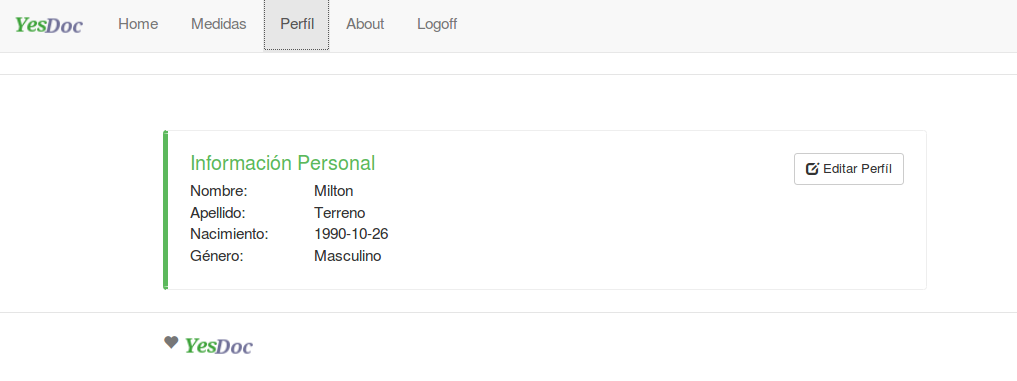
\includegraphics[width=1\textwidth]{img/tp1_parte2/1-perfil}
        \caption{Pantalla de perfil de usuario}
		\label{perfil}
    \end{figure}

\subsubsection{Creación de página de formulario de creación de perfil}      
Se generará el formulario necesario para que el usuario pueda cargar los datos personales antes nombrados. Se presentará una pantalla provisoria de inicio \textbf{Figura \ref{logeo}}  donde se le dará lo opción de logearse o de generar un nuevo perfil.
La opción de \textbf{Nuevo Perfil}, conducirá al usuario al formulario \textbf{Figura \ref{crear_perfil}} donde se realizarán las cargas respectivas de datos
      Para poder crear un nuevo perfil al usuario será necesario  acceder al recurso \texttt{/profiles/\{:d\}} de la API a través de un método \textbf{POST}
    \begin{figure}[h]
        \centering
        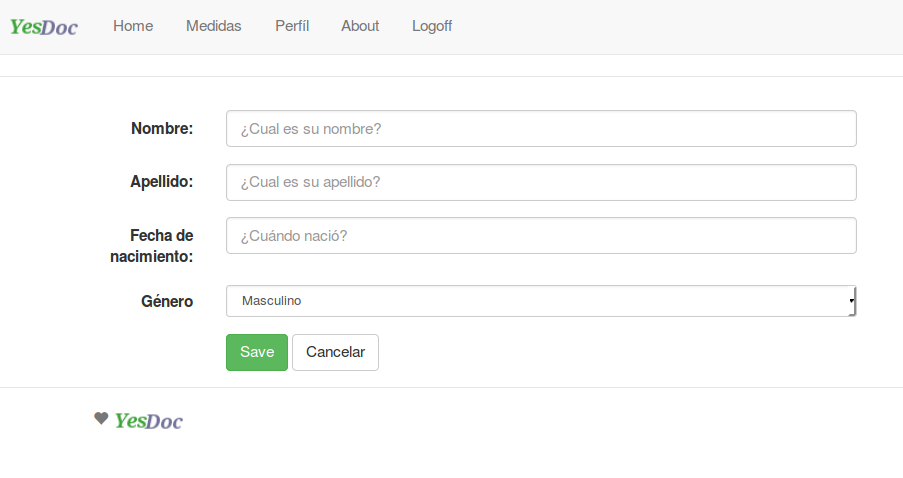
\includegraphics[width=1\textwidth]{img/tp1_parte2/1-crear_perfil}
        \caption{Formulario de creación de perfil}
		\label{crear_perfil}
    \end{figure}
    \begin{figure}[h]
        \centering
        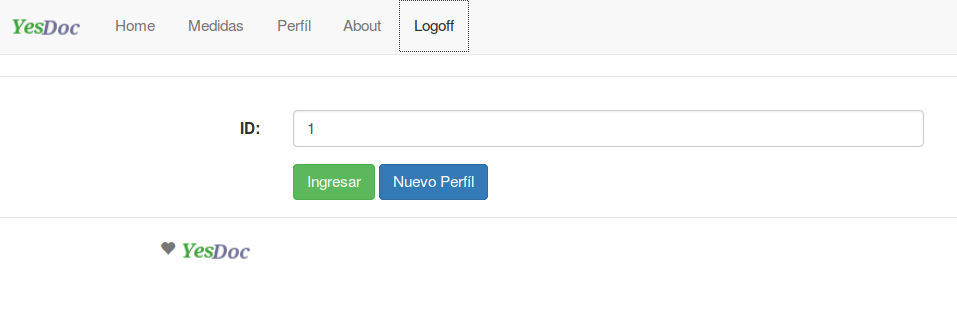
\includegraphics[width=1\textwidth]{img/tp1_parte2/1-logeo}
        \caption{Pantalla de logeo de usuario}
		\label{logeo}
    \end{figure}

\subsubsection{Creación de página de formulario de edición de perfil}      
\begin{figure}[h]
        \centering
        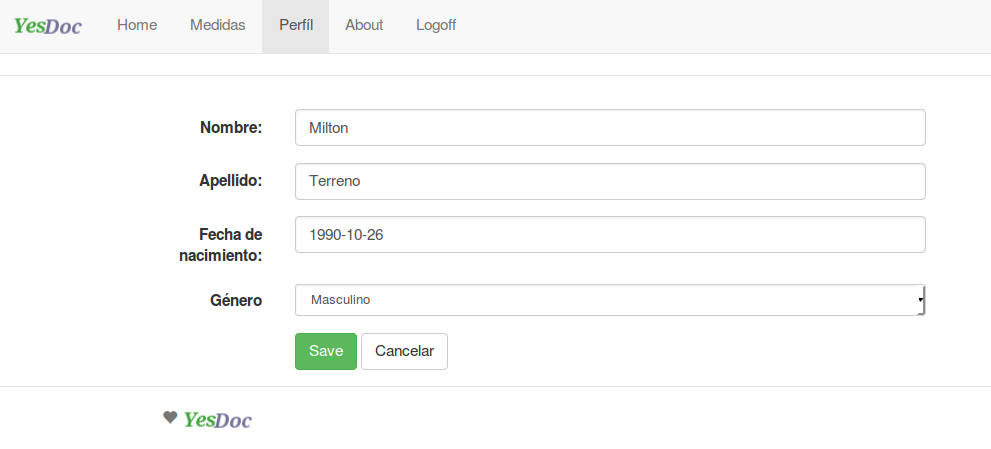
\includegraphics[width=1\textwidth]{img/tp1_parte2/1-editar_perfil}
        \caption{formulario de edición de perfil}
		\label{editar_perfil}
\end{figure}
Se generará el formulario necesario para que el usuario pueda modificar los datos personales antes nombrados. 
En la pantalla de perfil de usaurio \textbf{Figura \ref{perfil}} se le ofrecerá al usaurio la opción de \textbf{Editar Perfil} que lo redireccionará al formulario correspondiente a la edición del perfil, en los campos de dicho formulario se presentarán los datos del perfil, de este modo el usuario solo modificará el campo correspondiente
      Para poder guardar los nuevos datos del perfil al usuario será necesario  acceder al recurso \texttt{/profiles/\{:id\}} de la API a través de un método \textbf{PUT}

    
    
\subsection {Salidas del Sistema - Incrementos}

Luego de finalizado este user story se obtendrá como salida el logo correspondiente a la aplicación que se muestra en la \textbf{Figura \ref{logoYesDoc}}, y 4 pantallas que se detallarán a continuación:
\begin{enumerate}
	\item \textbf{Logeo de usuario:} \textbf{[Figura \ref{logeo}]} Desde esta pantalla el usuario podrá logearse  o crear un perfil nuevo
	\item \textbf{Creación de perfil:}\textbf{[Figura \ref{crear_perfil}]} Se le permitirá cargar aquellos datos que lo identifique nombre, apellido, fecha de nacimiento y género.
    \item \textbf{Presentación de la información personal:} \textbf{[Figura \ref{perfil}]} Aquí se mostrarán los datos personales del usuario (nombre, apellido, fecha de nacimiento y género.), brindándole la posibilidad de edición de los mismos.
    \item \textbf{Edición del perfil:}\textbf{[Figura \ref{editar_perfil}]} En esta pantalla se mostrará el formulario para realizar la edición correspondiente del perfil, los campos estarán precargados con los valores del perfil del usuario, para que éste los modifique según disponga.
\end{enumerate}



\clearpage	
\subsection{Planificación de pruebas}
\subsubsection{Criterios de aceptación}


\begin{center}
\begin{longtable}{|m{0.5cm}|m{4cm}|m{4cm}|m{4.5cm}|}
\hline \rowcolor[gray]{0.9}
	\multicolumn{4}{|c|}{\textbf{Criterio de aceptación}} \\
    \hline  \rowcolor[gray]{0.9}
        \multicolumn{1}{|c|}{\textbf{ID}} &
        \multicolumn{1}{c|}{\textbf{Contexto}} &
        \multicolumn{1}{c|}{\textbf{Evento}} &
        \multicolumn{1}{c|}{\textbf{Resultado}} \\
    \hline
        1&En caso de que el usuario exista & y este quiera ingresar al sistema & El sistema le mostrara sus datos personales\\ \hline
        2 &       Si el usuario no existe & y quiere loguearse & El sistema no le permitirá ingresar\\ \hline
        3 &       Si el usuario existe y no está logueado & y quiere ingresar a ver su perfil& El sistema no le permitirá ingresar y lo mantendrá en la pantalla de login\\ \hline
        4 &       Si el usuario existe & y quiere editar su perfil & El sistema le permitirá modificar cualquiera de sus datos personales\\ \hline
  \end{longtable}
\end{center}


\subsubsection{Pruebas de unidad - Casos de Prueba}


	{\scriptsize
    \begin{table}[h]
    \centering
	\begin{tabular}{|l|p{10cm}||}
    	\rowcolor[gray]{0.9}
	    \hline 
        \hline 
       
		\textbf{Caso de prueba} & \textbf{Consultar perfil de usuario existente} \\  \hline
	    \textbf{Descripción del escenario}& Nombre: Marita; Apellido Martinez; fecha de Nacimiento:2015-06-01; género: femenino\\ \hline
	    \textbf{Criterio de aceptación}&  \textbf{En caso de que el usuario exista y este quiera ingresar al sistema. El sistema le mostrara sus datos personales}\\ \hline
        \textbf{Datos de entrada}&  Id:3\\ \hline
        \textbf{Condiciones de  prueba}& Se necesita que esté previamente cargado el usuario "Marita Martinez". \\ \hline \hline
	\end{tabular}
        \caption{Caso de prueba para criterio de aceptación 1}
    \end{table}
	}
 
    	{\scriptsize
        \begin{table}[h]
        \centering
	\begin{longtable}{|p{4cm}|p{6cm}|p{5cm}|}
	    \hline  \hline \rowcolor[gray]{0.9} 
        \multicolumn{3}{||l|}{\textbf{Procedimiento de Prueba - ``Consultar perfil de usuario existente''}} \\
        \hline \rowcolor[gray]{0.9}
	    \textbf{Actor} & \textbf{Sistema}&\textbf{Resultado Esperado} \\  \hline
	   El usuario ingresa en el campo login el id:3 & & \\ \hline
        &El Sistema realiza una consulta a la API a partir del id:3 solicitando los datos de la instancia perfil específica&   \\ \hline
        &&Se muestra el  perfil de usuario con sus datos: Nombre: Marita; Apellido Martinez; fecha de Nacimiento:2015-06-01; género: femenino  \\ \hline
	    \end{longtable}
        \caption{Procedimiento de prueba para criterio de aceptación 1}
        \end{table}
	}
    
    {\scriptsize
	\begin{table}[h]
	\centering
	\begin{tabular}{|l|p{10cm}|}
	    \hline 
	    \textbf{Salida obtenida}&Se obtuvieron los datos que se detallaron previamente en ``Resultado esperado''\\ \hline
	    \textbf{Resultado}& \textbf{Correcto}\\ \hline
        \textbf{¿Qué fue mal?}& Nada\\ \hline      
        \textbf{Evidencia}&  \\ \hline
        \textbf{Seguimiento}& No es necesario ya que el caso de prueba no causó fallos \\ \hline
        \textbf{Estado}& \textbf{Terminado}\\ \hline        
        \textbf{¿Qué se puede mejorar?}& En una futura iteración se podría añadir el grupo sanguíneo y añadir un cartel de bienvenida al sistema \\ \hline              
	    \end{tabular}
        \caption{Resultado esperado para el criterio de aceptación 1}
    	\end{table}
	}
    

    %%%%%%%%   
    
\clearpage    
    
    {\scriptsize
	\begin{table}[h]
	\centering
	\begin{tabular}{||l|p{10cm}||}
    	\rowcolor[gray]{0.9}
	    \hline 
        \hline 
	    \textbf{Caso de prueba} & \textbf{Consultar perfil de usuario No existente} \\  \hline
	    \textbf{Descripción del escenario}&\\ \hline
	    \textbf{Criterio de aceptación}&\textbf{Si el usuario no existe y quiere loguearse. El sistema no le permitirá ingresar}\\ \hline
        \textbf{Datos de entrada}&  Id:64\\ \hline
        \textbf{Condiciones de  prueba}& No existe un usuario con id=64 \\ \hline \hline
	    \end{tabular}
        \caption{Caso de prueba para criterio de aceptación 2}
    	\end{table}
	}
    
    {\scriptsize
        \begin{table}[h]
        \centering
	\begin{longtable}{|p{4cm}|p{6cm}|p{5cm}|}
	    \hline  \hline \rowcolor[gray]{0.9} 
        \multicolumn{3}{||l|}{\textbf{Procedimiento de Prueba - ``Consultar perfil de usuario NO existente''}} \\
        \hline \rowcolor[gray]{0.9}
	    \textbf{Actor} & \textbf{Sistema}&\textbf{Resultado Esperado} \\  \hline
	   El usuario ingresa a loguearse con el id:64 & & \\ \hline
        & El Sistema realiza una consulta a la API a partir del id:64 solicitando los datos de la instancia perfil específica &   \\ \hline
        &El Sistema detecta que no existe un perfil con id:64&  Se mantiene al usuario en la vista de login\\ \hline
	    \end{longtable}
        \caption{Procedimiento de prueba para criterio de aceptación 2}
        
    	\end{table}
    }
    
    {\scriptsize
	\begin{table}[h]
	\centering
	\begin{longtable}{|l|p{10cm}|}
	    \hline 
	    \textbf{Salida obtenida}&El sistema permitió el ingreso a la interfaz de perfil, mostrando los datos vacíos\\ \hline
	    \textbf{Resultado}& \textbf{Fallido} \\ \hline
        \textbf{¿Qué fue mal?}& El sistema no le debería haber permitido al usuario ingresar\\ \hline      
        \textbf{Evidencia}& Imagen \ref{prueba2} \\ \hline
        \textbf{Seguimiento}&  En la Imagen \ref{correccionprueba2} se pueden ver las modificaciones que tuvieron que hacerse en el código del archivo login.js del controller para poder resolver el error descubierto, las líneas en rojo son las que se encontraban en un comienzo, las cuales producían error, y tuvieron que ser reemplazadas por las lineas marcadas en verde para que las pruebas pasen. También se puede ver en las figura \ref{Codigoinicialprueba2} como se encontraba el código inicialmente.\\ \hline
        \textbf{Estado}& \textbf{Terminado \& Corregido}\\ \hline        
        \textbf{¿Qué se puede mejorar?}& Se corrigieron los errores pero en otra iteración se podría añadir carteles de advertencia, esto se verá en los sprint relacionados a la seguridad\\ \hline              
     
	    \end{longtable}
        \caption{Resultado esperado para el criterio de aceptación 2}
    	\end{table}
	}
    
\begin{figure}[h]
  \centering
  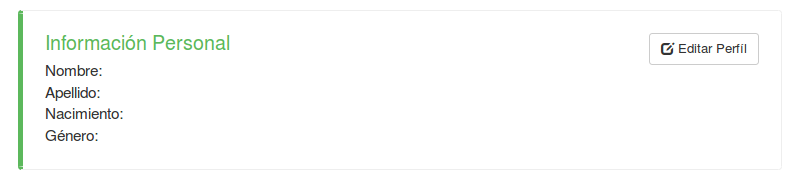
\includegraphics[width=.8\textwidth]{img/tp1_parte2/1-prueba_2}
  \caption{error en la pruebas 2}
  \label{prueba2}
\end{figure}

\begin{figure}[h]
  \centering
  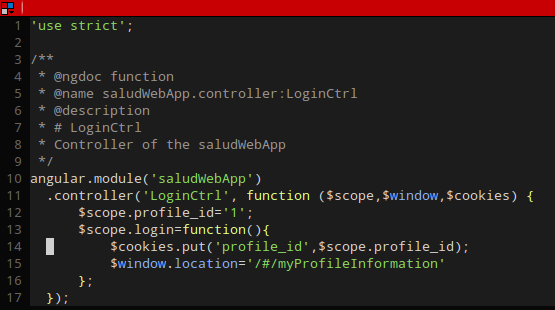
\includegraphics[width=.8\textwidth]{img/tp1_parte2/1-codigo_prueba_2}
  \caption{Código utilizado inicialmente para el login}
  \label{Codigoinicialprueba2}
\end{figure}


\begin{figure}[h]
  \centering
  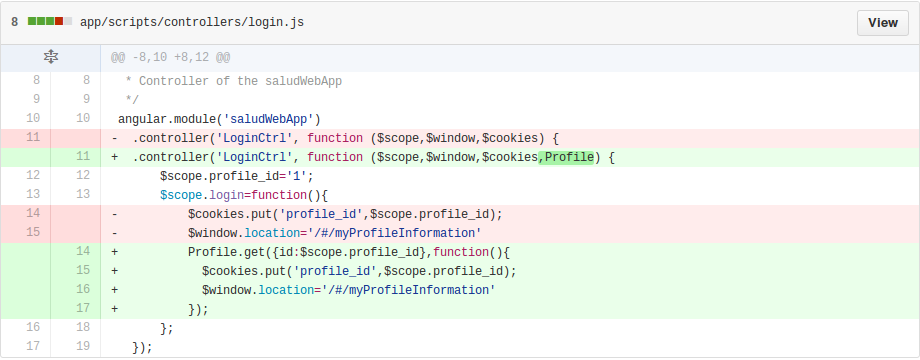
\includegraphics[width=.8\textwidth]{img/tp1_parte2/1-correccion_prueba_2}
  \caption{Correcciones de los error detectados en la pruebas 2}
  \label{correccionprueba2}
\end{figure}

\clearpage
    %%%%%%%%%%%%%%%%%%%%%%

{\scriptsize
	\begin{table}[h]
	\centering
	\begin{tabular}{||l|p{10cm}||}
    	\rowcolor[gray]{0.9}
	    \hline 
        \hline 
	    \textbf{Caso de prueba} & \textbf{Ingresar al sistema sin loguearse} \\  \hline
	    \textbf{Descripción del escenario}& no son necesarios\\ \hline
	    \textbf{Criterio de aceptación}&\textbf{Si el usuario existe y no está logueado y quiere ingresar a ver su perfil, el sistema no le permitirá ingresar y lo mantendrá en la pantalla de login}\\ \hline
        \textbf{Datos de entrada}&  ninguno\\ \hline
        \textbf{Condiciones de  prueba}& el usuario no se loguea \\ \hline \hline
	    \end{tabular}
        \caption{Caso de prueba para criterio de aceptación 3}
    	\end{table}
	}
    
    {\scriptsize
	\begin{table}[h]
    \centering
	\begin{longtable}{|p{5cm}|p{5cm}|p{4cm}|}
	    \hline \hline \rowcolor[gray]{0.9}
        \multicolumn{3}{||l|}{\textbf{Procedimiento de Prueba - ``Ingresar al sistema sin loguearse''}} \\
        \hline 
        \rowcolor[gray]{0.9}
	    \textbf{Actor} & \textbf{Sistema}& \textbf{Resultado Esperado} \\  \hline
	   El usuario selecciona la pestaña de ``perfil'' para ingresar a ver su perfil (sin antes haberse logueado) & & \\ \hline
        & El sistema valida que exista una cookie con las sesión creada&   \\ \hline
        &El Sistema no encuentra una cookie existente y no hace nada&  Se mantiene al usuario en la vista de login\\ \hline
	    \end{longtable}
        \caption{Procedimiento de prueba para criterio de aceptación 3}
    	\end{table}
    }
    
    {\scriptsize
	\begin{table}[h]
	\centering
	\begin{longtable}{|l|p{10cm}|}
	    \hline 
	    \textbf{Salida obtenida}&El sistema mantuvo al usuario no logueado en la ventana de login, garantizando que no ingrese al sistema\\ \hline
	    \textbf{Resultado}& \textbf{Correcto}\\ \hline
        \textbf{¿Qué fue mal?}& Todo salio como se esperaba\\ \hline      
        \textbf{Evidencia}& para esta prueba no es necesaria \\ \hline
        \textbf{Seguimiento}& No es necesario ya que el caso de prueba no causó
fallos \\ \hline
        \textbf{Estado}& \textbf{Terminado}\\ \hline        
        \textbf{¿Qué se puede mejorar?}& En otra iteración se podría añadir carteles de advertencia, esto se verá en los sprints relacionados a la seguridad.\\ \hline              
	    \end{longtable}
        \caption{Resultado esperado para el criterio de aceptación 3}
    	\end{table}
	}
    

\clearpage
    %%%%%%%%%%%%%%%%%%%%%%%%%%%%

    {\scriptsize
	\begin{table}[h]
	\centering
	\begin{tabular}{||l|p{10cm}||}
    	\rowcolor[gray]{0.9}
	    \hline 
        \hline 
	    \textbf{Caso de prueba} & \textbf{Editar perfil} \\  \hline
	    \textbf{Descripción del escenario}&Nombre: Marita; Apellido Martinez; fecha de Nacimiento:2015-06-01; género: femenino; id:3\\ \hline
	    \textbf{Criterio de aceptación}& \textbf{Si el usuario existe y quiere editar su perfil, el sistema le permitirá modificar cualquiera de sus datos personales}\\ \hline
        \textbf{Datos de entrada }& datos modificados nombre: Marita Emilce\\ \hline
        \textbf{Condiciones de  prueba}&  usuario con id:3 logueado \\ \hline \hline
	    \end{tabular}
        \caption{Caso de prueba para criterio de aceptación 4}
    	\end{table}
	}
    
    {\scriptsize
	\begin{table}[h]
    \centering
	\begin{longtable}{|p{5cm}|p{5cm}|p{4cm}|}
	    \hline \hline \rowcolor[gray]{0.9}
        \multicolumn{3}{||l|}{\textbf{Procedimiento de Prueba - ``Editar perfil''}} \\
        \hline 
        \rowcolor[gray]{0.9}
	    \textbf{Actor} & \textbf{Sistema}& \textbf{Resultado Esperado} \\  \hline
	   El usuario presiona sobre el botón``editar perfil'' & & \\ \hline
        & El Sistema realiza una consulta a la API a partir del id:3 para traer los datos del perfil y precargar el formulario &   \\ \hline
        & &  Se muestra un formulario con los datos del usuario para que sean modificados\\ \hline
        El usuario modifica su nombre y añade un segundo nombre Emilce&& \\ \hline
        &El sistema carga los nuevos datos a la API a través del método PUT&\\ \hline
        &El sistema redirecciona al usuario a la vista de perfil de usuario&Se muestra el perfil con sus datos y el nuevo nombre ingresado\\ \hline
	    \end{longtable}
        \caption{Procedimiento de prueba para criterio de aceptación 4}
    	\end{table}
    }
    
    {\scriptsize
	\begin{table}[h]
	\centering
	\begin{tabular}{|l|p{10cm}|}
	    \hline 
	    \textbf{Salida obtenida}& El formulario con los datos se mostraron correctamente\\ \hline
	    \textbf{Resultado}& \textbf{Correcto}\\ \hline
        \textbf{¿Qué fue mal?}& nada\\ \hline      
        \textbf{Evidencia}& En la Imagen \ref{prueba4} se puede ver el formulario con los datos precargados y en el Json \ref{JsonProfile} que contiene los nuevos datos los cuales accedemos a partir de la URL \begin{lstlisting} 
https://yesdoc-api.herokuapp.com/profiles/3 \end{lstlisting}\\ \hline
        \textbf{Seguimiento}& No es necesario ya que el caso de prueba no causó
fallos
\\ \hline
        \textbf{Estado}& \textbf{Terminado}\\ \hline        
        \textbf{¿Qué se puede mejorar?}& \\ \hline              
	    \end{tabular}
        \caption{Resultado esperado para el criterio de aceptación 4}
    	\end{table}
	}
\clearpage

\begin{figure}[h]
  \centering
  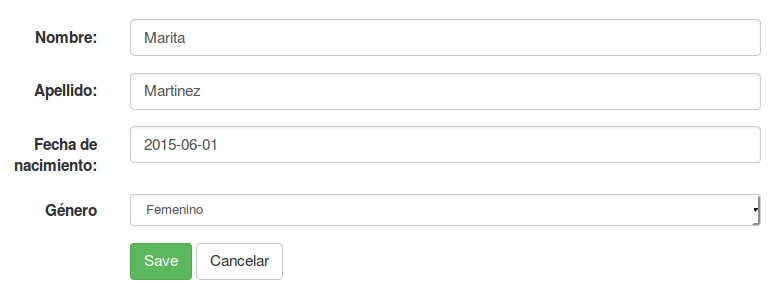
\includegraphics[width=.8\textwidth]{img/tp1_parte2/1-prueba_4}
  \caption{Prueba 4}
  \label{prueba4}
\end{figure}

\begin{lstlisting}[language=json,firstnumber=1,  breaklines=true, caption= Json del perfil id:3 modificado, label=JsonProfile]
{
 "resource": {
    "gender":{
            "description": null,
            "id": 2,
            "name": "Femenino"
        },
        "first_name": "Marita Emilce",
        "last_name": "Martinez",
        "id": 3,
        "birthday": "2015-06-01"
    }
}
\end{lstlisting}

\clearpage
    %%%%%
    
    


    
    %%%%
    \clearpage
\subsubsection{Pruebas de integración entre módulos del Sistema}
Estas pruebas se realizarán más adelante, en futuros sprints.
\subsubsection{Pruebas de carga}
En este sprint no se realizarán este tipo de pruebas.
\subsubsection{Pruebas de seguridad por niveles de usuario}
En este sprint no se realizarán este tipo de pruebas, ya que la seguridad será un tema a tratar más adelante.

\subsection{Pruebas ejecutadas}
Aquí se realizará una conclusión general de lo que se descubrió en las pruebas.
	\begin{itemize}
		\item \textbf{¿Qué fue bien?}
        	\begin{itemize}
				\item Los datos de usuario se mostraron correctamente, además al cargar  los datos no se tuvo inconveniente alguno.
			\end{itemize}
   		\item \textbf{¿Qué se mejoró?}
        	\begin{itemize}
				\item \textbf{Cerrado}  Se detecto que cuando un usuario inexistente iniciaba sesión, podía ingresar al módulo de perfil, en este módulo no se mostraban los datos, ya que no existía  el usuario, pero no era correcto que esto sucediera.
                \item \textbf{Cerrado} Se encontraron problemas  con los nav's, los cuales sólo se marcaban como seleccionados cuando se presionaban y esto no nos servía para los casos en los que había que redireccionar. Se solucionó utilizando Angular Strap.
                
			\end{itemize}
   		\item \textbf{¿Qué se puede mejorar?}
        	\begin{itemize}
				\item \textbf{Abierto} Al finalizar el Sprint se vio necesario implementar un ítem que indique el grupo sanguíneo de la persona.
                \item \textbf{Abierto} Se podría arreglar la forma de seleccionar las fechas en el caso de la "fecha de nacimiento".
                \item \textbf{Abierto} Se deberá añadir, en los sprint relacionados a seguridad, los carteles de advertencia correspondientes.
                \item \textbf{Abierto} En próximas iteraciones deberá añadirse el grupo sanguíneo de la persona
                \item \textbf{Abierto} En próximas iteraciones deberá añadirse un cartel de bienvenida del usuario al sistema.
			\end{itemize}
    \end{itemize}